\documentclass[12pt]{article}


\usepackage{graphicx}
\graphicspath{ {./img/} }

\usepackage[margin=1.25in]{geometry}

\usepackage[english,ngerman]{babel}

% box for functions
\usepackage[dvipsnames]{xcolor}
\usepackage[most]{tcolorbox}
\usepackage{hyperref}
\newtcolorbox{mybox}[2][]{%
  attach boxed title to top left
               = {yshift=-8pt},
  colback      = blue!5!white,
  colframe     = blue!75!black,
  fonttitle    = \bfseries,
  colbacktitle = gray!85!black,
  title        = #2,#1,
  enhanced,
}


\author{\\ Burenko Anton \\ s76905 \\ \\ \\ Prof. Dr. Wolfgang Oertel \\ 
Computergrafik 1 \\ \\
}

\date{Wintersemester 2018/19}
\title{Belegarbeit\\ "Sunset Pagoda"}

\begin{document}
\selectlanguage{ngerman}

\maketitle

\pagebreak

\tableofcontents

\pagebreak

\section{Aufgabenstellung}
Schreiben Sie ein Programm in C/C++, das unter Verwendung von OpenGL, Vertex- und
Fragment-Shadern folgende Aufgaben realisiert. \\ \\
\textbf{Aufgabe 1}: \\
Geometrische Objekte: Erzeugen Sie eine interaktive zeitlich animierte Szene mit mehreren
unterschiedlichen farblichen und texturierten dreidimensionalen geometrischen Objekten. \\ \\
\textbf{Aufgabe 2}: \\
Beleuchtung: Beleuchten Sie die Szene mit mehreren Lichtquellen so, dass auf den Objekten
unterschiedliche Beleuchtungseffekte sichtbar werden. \\ \\
\textbf{Aufgabe 3}: \\
Ansicht: Stellen Sie die Szene gleichzeitig in verschiedenen Ansichten und Projektionen in
mehreren Viewports des Anzeigefensters dar. \\ \\
\textbf{Aufgabe 4}: \\
Programm: Stellen Sie das komplette Programm in Quelltextform als Visual-Studio-C++ -
Projekt und in ausführbarer Form als exe-File derart bereit, dass die Lauffähigkeit auf den
Computern des Praktikumslabors der Lehrveranstaltung gewährleistet ist. \\ \\
\textbf{Aufgabe 5}: \\
Dokumentation: Fertigen Sie eine Systemdokumentation in Form eines pdf-Dokumentes von
etwa 10 Seiten an, die Deckblatt, Gliederung, Aufgabenbeschreibung, Lösungsansatz,
Lösungsumsetzung, Installations- und Bedienungsanleitung, einige Bildschirm-Snapshots,
Probleme, Ergebnisse, Literatur- und Quellenverzeichnis enthält. \\ \\
\textbf{Aufgabe 6}: \\
Abgabe: Demonstrieren Sie die Ergebnisse der Aufgaben 4 und 5 an einem Computer des
Praktikumslabors der Lehrveranstaltung und übergeben Sie diese in einem Verzeichnis
$"Name\_Vorname\_Bibliotheksnummer"$. \\ \\
\textbf{Zeitplan}: \\
Die Ausgabe der Aufgabenstellung erfolgt zu Beginn der Lehrveranstaltungszeit. Die Abgabe
der Ergebnisse erfolgt spätestens zum Ende der Lehrveranstaltungszeit. \\

\pagebreak
\section{Bedienungsanleitung}
Das Programm verwendet OpenGL und Visual Studio, um die Szene zu kompilieren und auszuführen. Die Hauptbibliothek dafür sind opengl32, freeglut, glew32, FreeImage. Die müssen vorher durch Linker und C++ - compiler gebunden sein.

\bigbreak



\bigbreak

Die Texturen und alle .cpp sowie Headers und Shaders Dateien müssen in dem Verzeichnis "Programme" gespeichert werden. Welche Texturen es gibt kann man im Punkt "Texture" detaliert lesen.

\section{Functionen}
\begin{mybox}[colback=lightgray]{main}
\textbf{int main(int argc, char$**$ argv)} \\
initialisiert das Program, bestimmt Window Size, Namen, und bindet Fuktionen für Aufruf(z.B. keyboard, display).
\end{mybox}

\begin{mybox}[colback=white]{generateBox24}
\textbf{void generateBox24()} \\
generate Positionen, Farben, Normalen und Texturekoordinaten für einen Würfel. 
Außerdem speichert die für VAO und Position Buffers.
\end{mybox}
\begin{mybox}[colback=white]{drawBox24}
\textbf{void drawBox24()} \\
zeichnet den Würfel von gegebenen Positionen.
\end{mybox}

\begin{mybox}[colback=white]{generatePiramideExTop}
\textbf{void generatePiramideExTop()} \\
generate Positionen, Farben, Normalen und Texturekoordinaten für einen Dachobject. 
Außerdem speichert die für VAO und Position Buffers.
\end{mybox}
\begin{mybox}[colback=white]{drawPiramideExTop}
\textbf{void drawPiramideExTop()} \\
zeichnet das Dachobject von gegebenen Positionen.
\end{mybox}

\begin{mybox}[colback=white]{generatePiramide}
\textbf{void generatePiramide()} \\
generate Positionen, Farben, Normalen und Texturekoordinaten für eine Piramide. 
Außerdem speichert die für VAO und Position Buffers.
\end{mybox}
\begin{mybox}[colback=white]{drawPiramide()}
\textbf{void drawPiramide()} \\
zeichnet eine Piramide von gegebenen Positionen.
\end{mybox}

\begin{mybox}[colback=white]{init}
\textbf{void init()} \\
initialisiert Shaders, Texturen, Tiefenpuffer, ruft alle generate* Funktionen und alle Locations für $uniform$s
\end{mybox}

\begin{mybox}[colback=white]{lichtBerechnung}
\textbf{void lichtBerechnung()} \\
berechnet ModelViewProjection, ModelView und NormalMatrix und übergibt die Variablen als $uniform$s.
\end{mybox}

\begin{mybox}[colback=white]{drawFigures}
\textbf{void drawFigures()} \\
wählt richtige Texturen und zeichnet alle Objecte der Szene.
\end{mybox}

\begin{mybox}[colback=white]{display}
\textbf{void display()} \\
stellt View, Viewports bzw. drawFigures
\end{mybox}

\begin{mybox}[colback=white]{keyboard}
\textbf{void keyboard(unsigned char theKey, int mouseX, int mouseY)} \\
implementiert keyboard interaction(siehe Interaction).
\end{mybox}

\begin{mybox}[colback=white]{mouse}
\textbf{void mouse(int mouseX, int mouseY)} \\
implementiert mouse interaction(siehe Interaction).
\end{mybox}

\pagebreak

\section{Viewports}
In der Szene sind 2 Viewports aktiv.
\bigbreak
\subsection{Viewport von Sonne}
Das Viewport kann man links sehen. Die "Kamera" bewegt sich mit der Sonne zusammen nach oben und unter. Aus dem Sicht kann man sehr gut das Spotlicht sehen. 

\subsection{Einstellbares Viewport}
Das Viewport kann man rechts sehen. Die "Kamera" bewegt sich durch Bewegen vom Maus des Benutzers. Aus dem Sicht kann man alles sehen. Außerdem ist es mit dem Viewport möglich das Richtungslicht auf dem Dach bemerken. 

\begin{center}
\includegraphics[width=15cm, height=7.5cm]{viewports}
\end{center}

\pagebreak

\section{Figure}
Für diese Szene sind 3 Figuren verwendet: ein Würfel, eine Piramide und einen Pyramidenstumpf. Alle Figuren haben eine neutrale Farbe, die danach mit einem Texture überdeckt wird. \\
\subsection{Würfel}
Der Würfel wird für Grass, Sonne und Gebäudeblocke verwendet. \\ \\
\begin{center}
\includegraphics[width=6cm, height=6cm]{blocks}
\includegraphics[width=2cm, height=2cm]{sunSCR}
\includegraphics[width=6cm, height=6cm]{floorSCR}
\end{center}
\subsection{Piramide}
Die Piramide ist nur für Dach von Pagode verwendet.
\subsection{Pyramidenstumpf}
Der Pyramidenstumpf ist für den Zwischendach von Pagode verwendet. \\\\
\includegraphics[width=6cm, height=5cm]{roofsSCR}

\pagebreak

\section{Texture}
Es gibt folgende Texturen: roof, wall, grass and sun. \\
\textbf{roof:}
\begin{center}
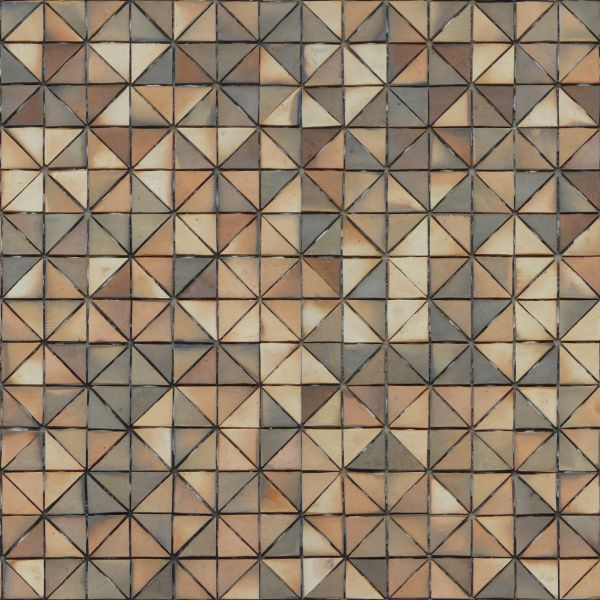
\includegraphics[width=4cm, height=4cm]{roof} \\
\end{center}
\textbf{wall:}
\begin{center}
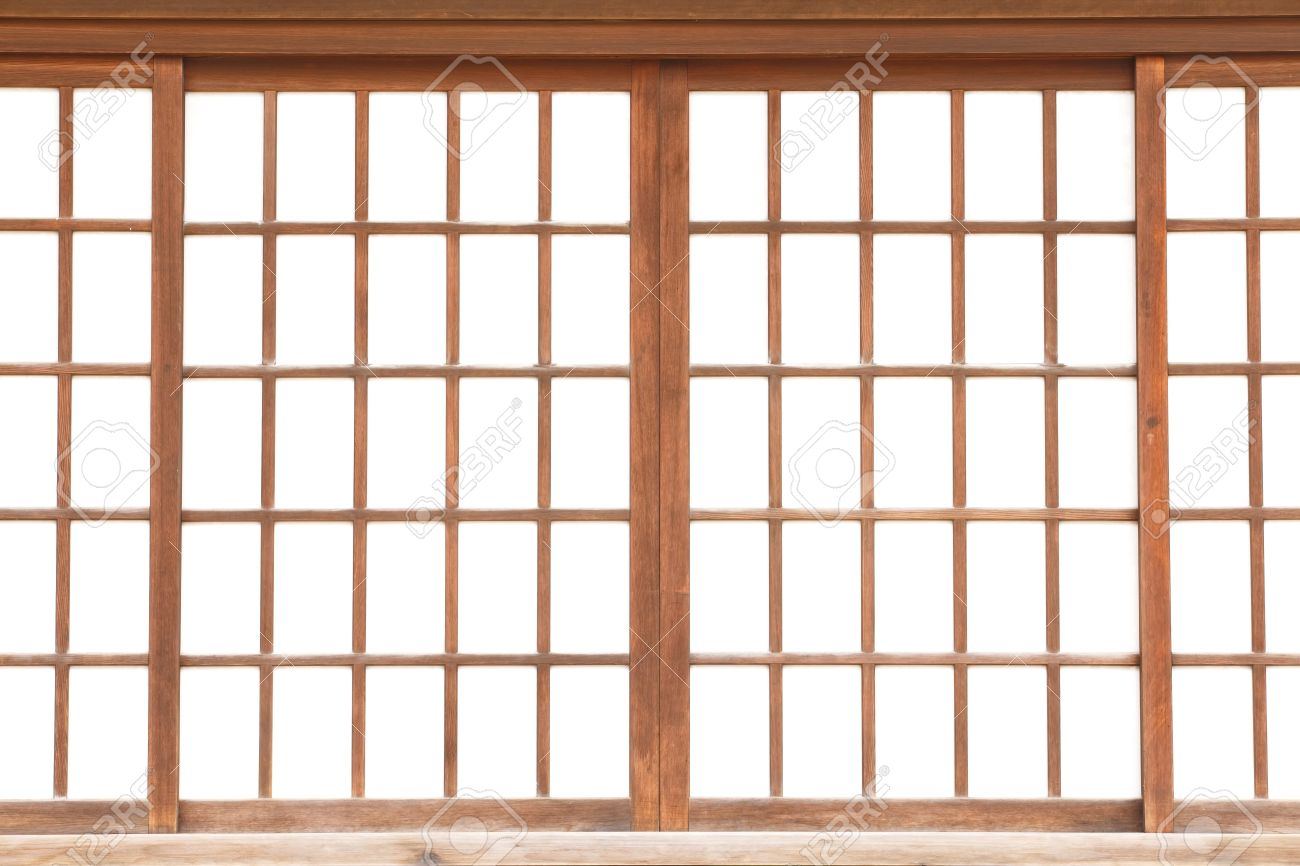
\includegraphics[width=8cm, height=4cm]{japwall} \\
\end{center}
\textbf{grass:}
\begin{center}
\includegraphics[width=4cm, height=4cm]{grass} \\
\end{center}
\textbf{sun:}
\begin{center}
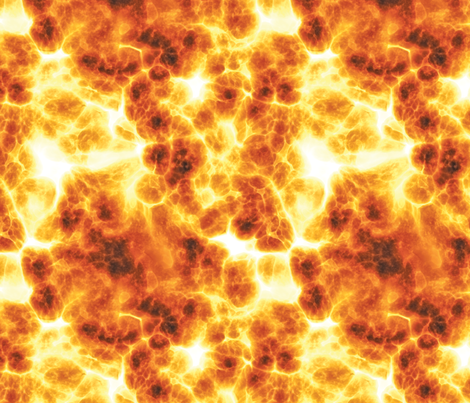
\includegraphics[width=4cm, height=4cm]{sun}
\end{center}

\pagebreak
\section{Light}
Die Szene enthält drei Lichtquellen: Ambiente licht, Spotlicht und Richtungslicht.
Alle Lichtquellen sind in dem Fragment Shader implementiert.
\subsection{Ambiente Licht}
\paragraph{Position} Ambiente Licht gibt es überall auf der Szene. \\\\
In dieser Szene wechselt es die Farbe von Weiß auf Rot und umgekehrt(siehe \textbf{Animation}), um den Sonnenuntergang zu simulieren.
\subsection{Spotlicht}
\paragraph{Position} Bewegt sich mit der Sonne zusammen.\\\\ 
Das Spotlicht sieht wie ein Lichtkreis von der Richtung von der Sonne aus. Die Lichtquelle bewegt sich mit dem Licht zusammen (siehe \textbf{Animation}).
Die Weiße Farbe wird vom Zenter bis Rand immer schwacher. \\\\ 
\includegraphics[width=6cm, height=6cm]{spotlight}
\pagebreak
\subsection{Richtungslicht}
\paragraph{Position} $(4,4,4)$ Orientiert von der Sonne rechts oben.\\\\ 
Richtungslicht kann man sehr gut als Blicke auf dem Dach beachten. Die Blicke kann man nur auf zwei Seiten sehen, weil das Licht nur aus einer Seite die Pagode beleuchtet. Am besten ist es zu sehen wenn man das Spotlicht ausmacht (siehe \textbf{Interaction}).\\\\ 
\includegraphics[width=6cm, height=6cm]{richtungslicht}
\includegraphics[width=6cm, height=6cm]{richtungslicht1}
\paragraph{Richtungslicht und Spotlicht} zusammen \\\
\includegraphics[width=12cm, height=6cm]{spotANDrichtungslicht}


\pagebreak

\section{Animation}
Animation kann man schon am Anfang der Szene sehen. Die Sonne bewegt sich an der Y-Achse nach oben bzw. unten. \\
Außerdem ändert sich die Farbe dabei, um Sonnenuntergang zu simulieren.
Wenn die Sonne schon unter Niveau vom Grass-block bzw. der Erde ist wird die Farbe rot. \\\\
\begin{center}
Sonne oben\\
\includegraphics[width=12cm, height=6cm]{suntop} 
\bigbreak
Sonne unten\\
\includegraphics[width=12cm, height=6cm]{sunbottom}
\end{center}

\pagebreak

\section{Interaction}
Die Szene kann man mit Mouse sowie mit Keyboard steuern.\\\\
Berechnungen dazu findet man in Funktionen keyboard sowie mouse.\bigbreak
\textbf{Keyboard mapping} \\\\
Z ... kleiner \\\\
V ... größer \\\\
D ... Tiefenbuffer an/aus \\\\
1 ... Richtungslich und Ambiente Licht an/aus \\\\
2 ... Spotlicht an/aus

\bigbreak
\section{Quellenverzeichnis}
\paragraph{OpenGL SuperBible} by Sellers, Wright Jr., Haemel

\paragraph{OpenGL Programming Guide}: The Official Guide to Learning OpenGL, Version 2 

\paragraph{Computergraphik 1 Vorlesungsmaterial} by Prof. Dr. Wolfgang Oertel 

\end{document}
\pagebreak
 